\documentclass[a4paper,14pt,spanish]{article}
\usepackage{mathtools}
\usepackage[spanish,activeacute]{babel}
\usepackage[utf8]{inputenc}
\usepackage{color}
\usepackage{graphicx}
\parindent 0em
\newcommand{\textoverline}[1]{$\overline{\mbox{#1}}$}
\newcommand{\tab}{\hspace*{2em}}
\usepackage[margin=1in]{geometry}
\newcommand{\HRule}{\rule{\linewidth}{0.5mm}}


\begin{document}
\begin{titlepage}
\begin{center}
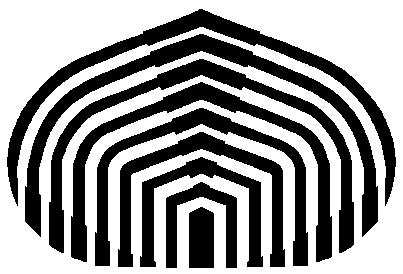
\includegraphics[scale=0.25]{res/USB.jpg}~\\[1cm]

\textsc{\LARGE Universidad Simón Bolívar}\\[1.5cm]
\textsc{\Large CI-5651 : Diseño de Algoritmos}\\[1.5cm]

\HRule \\[0.4cm]
{ \huge \bfseries Greedy\\[0.4cm] }

\HRule \\[1.5cm]
\begin{minipage}{0.4\textwidth}
\begin{flushleft} \large
\emph{Estudiantes:}\\
Melecio Ponte, 08-10993 \\
Gabriel Formica, 10-11036 \\
\end{flushleft}
\end{minipage}
\begin{minipage}{0.4\textwidth}
\begin{flushright} \large
\emph{Prof:} \\
Guillermo Palma \\
Alejandro Flores \\

\end{flushright}
\end{minipage}

\vfill
{\large \today}
\end{center}
\end{titlepage}

\tableofcontents
\newpage

\setlength\parindent{24pt}

\section{Problema 1}
Sean N oficinas, M modems; U costo por metro de cables regular, V costo por metro de cable especial, y R metros máximo
que pueden hacerse con una conexión regular;
el problema 1 demanda minimizar los costos totales de conectar las N oficinas a internet. Esto lo hacemos calculando M componentes
conexas, en donde cada componente sea un árbol mínimo cobertor. El pseudo-código de la solución \emph{para cada caso de prueba} es el siguiente:
    \begin{enumerate}
        \item Calcular todos los arcos posibles en el grafo, en donde cada arco tiene un peso
              que es igual a la distancia Euclideana de ambos nodos, cuidando además de no agregar arcos ya agregados:
              esto se hace en total de visitas igual $\displaystyle\sum\limits_{i=1}^{n-1} i = \frac{n(n-1)}{2}$, que conlleva a $O(n^2)$
        \item Se ordenan los arcos ascendentemente, sea \texttt e la cantidad de arcos generados, se tiene $O(e\log{}e)$ usando \emph{sort} de \texttt {STL}
        \item Se realiza un Kruskal donde la condición de parada es que la cantidad de componentes conexas, es igual a M
        \item El Kruskal retornará un par de enteros que indicará los metros de cables regulares (p1) y los metros de cables especiales (p2), respectivamente.
        \item Calcular (p1 * U) y (p2 * V)
    \end{enumerate}

Se usó además UnionFind Disjoint set como estructura para hacer las operaciones necesarias en Kruskal. Dicha estructura tiene dos optimaciones basadas en dos heurísticas:
{\bf compresión de camino} y {\bf unión por ranking}.

\subsection{Conclusión}
Dado que los arcos de las M componentes conexas son exactamente los arcos dados por Kruskal en algún punto de la iteración, y dado que Kruskal es óptimo,
entonces el algoritmo greedy es óptimo. La complejidad total del algoritmo es $O(n^2)$ + $O(e\log{}e)$ + $O(e*alpha(2e,n))$ que es igual
a $O(n^2 + e\log{}e)$, donde \texttt alpha es la función inversa de la función de \texttt Ackermann.

\clearpage
\section{Problema 2}
Sea N el número de oficinas en una red de computadoras y el par $\displaystyle x, y$ la represetanción de una conexión entre las oficinas $\displaystyle x$ y $\displaystyle y$. Dada una serie de instrucciones a realizar sobre los datos, se requieren dos operaciones:
\begin{itemize}
    \item \texttt{Q}: Se debe calcular el número de nodos que no se pueden conectar entre sí.
    \item \texttt{R X}: Se debe eliminar del conjunto de arcos el arco \texttt{X}-esimo arco.
\end{itemize}

La resolución de la operación \texttt{Q} se hace mediante la aplicación de la estrategia \emph{greedy} del algoritmo de Kruskal pero con dos distinciones importantes: No se tiene pesos en los arcos, por lo que no hay necesidad de ordenarlos y no siempre se busca obtener un arbol mínimo cobertor (salvo en los casos en los que todos los arcos estén) sino más bien el bosque de árboles que existe en algún punto intermedio del algoritmo.

Para esto resulta evidentemente conveniente el uso de la estructura de conjuntos disjuntos (\emph{disjoint sets}) que se implementa bajo el nombre de \emph{UnionFind Disjoint}, cuyas optimizaciones se explicaron en el problema anterior.

El cálculo del número de pares de nodos que están desconectados entre sí se logra de la siguiente manera: Dado un conjunto de vértices $\displaystyle V$, conjunto de arcos que conforman $\displaystyle X$ componentes conexas, se tiene que el conjunto de pares desconectados entre sí $\displaystyle x = \frac{|V|(|V|-1)}{2} - \sum\limits_{i=1}^{X}\frac{|X_i|(|X_i|-1)}{2} $.

Es decir, la cantidad de pares de nodos desconectados entre sí se calcula sabiendo la cantidad de arcos posibles y restándoles aquellos que sí existen, ya sea de manera directa o indirecta.

El algoritmo entonces procede de la siguiente manera:

\begin{enumerate}
    \item Se tiene un conjunto con los arcos sin orden en particular.
    \item Se inicializa el UnionFind Disjoint \emph{set} incialmente con tantos elementos como vértices.
    \item Se crea un diccionario \emph{table} inicialmente vacio cuya clave es un nodo representante de su conjunto y su valor el tamaño de la componente conexa asociada.
    \item Para cada arco \emph{(x, y)}:
    \begin{enumerate}
        \item Si x no está en el mismo conjunto que y, se unen en \emph{set}.
        \item Se guarda en \emph{table} el tamaño de la componente conexa cuyo representante es \emph{y}.
    \end{enumerate}
    \item Se itera sobre \emph{table} para calcular la solución.
\end{enumerate}

\subsection{Conclusión}
La solución parte de los siguientes principios:
\begin{itemize}
    \item Encontrar las componentes conexas y sus tamaños permite de manera constante encontrar la cantidad de pares no conectados entre sí.
    \item El algoritmo de Kruskal y la estructura de conjuntos disjuntos provee una estrategia \emph{greedy} para encontrar las componentes conexas de un arbol añadiendo la ventaja de que, al no haber pesos involucrados, no hay que ordenar arcos ni descartar arcos que no sean parte del árbol.
    \item La operación \texttt{R X} funciona con complejidad constante ya que consiste simplemente en eliminar un elemento de una lista indexada y por ende su análisis se excluye cayendo la prioridad sobre la operación \texttt{Q}.
\end{itemize}

Dado $\displaystyle e$ arcos y $\displaystyle c$ componentes conexas, la complejidad del algoritmo entonces es  $O(e*alpha(n)*log(c))$ + $O(c)$ que es $O(e*log(c))$ que consiste en el tiempo de recorrer la lista de arcos, hacer las busquedas y uniones correspondientes en el conjunto disjunto y recorrer el diccionarios de componentes para calcular la solución.



\clearpage
\section{Problema 3}
Sea N el número de actividades que un empleado puede realizar, y $\displaystyle x_i, y_i$ el tiempo de inicio y
fin de la i-ésima actividad, respectivamente. El pseudo-código de la solución \emph{para cada caso de prueba} es el siguiente:
    \begin{enumerate}
        \item Ordenar las actividades que terminen primero: esto es, ascendentemente por su $\displaystyle y_i$. Esto se hace en $O(N\log{}N)$ usando
              \texttt STL
        \item Inicializar última\_actividad = 0, total\_actividades = 0
        \item Para cada actividad en la lista de actividades
            \begin{enumerate}
                \item si la actividad comienza después de última\_actividad
                    \begin{enumerate}
                        \item total\_actividad++
                        \item última\_actividad = actividad.y (donde actividad.y es el igual al tiempo final de una actividad)
                    \end{enumerate}
            \end{enumerate}
    \end{enumerate}

\subsection{Conclusión}
La idea es tratar de hacer aquellas actividades que terminen antes. El algoritmo greedy dará la mayor cantidad de actividades que pueden hacerse,
y la demostración es la siguiente:

Supongamos que nuestra solución greedy realiza solo k actividades $\displaystyle a_1, a_2, a_3,..,a_k$, y que la solución óptima
realiza N $>$ K actividades, en donde las primeras $\displaystyle a_1, a_2, a_3,..,a_k$, son las mismas actividades que la solución greedy realiza y que además, contiene $\displaystyle a_{k+1}, a_{k+2}$,.., an.
Dado que la solución greedy va agregando aquellas actividades que van terminando antes, entonces todas aquellas actividades después del tiempo K que pudieron ser
agregadas por la solución óptima, serán agregadas por la solución greedy.

La complejidad del algoritmo es $O(N\log{}N + N)$ = $O(N\log{}N)$ que es el tiempo en ordenar la lista de actividades más recorrer dicha lista.

\clearpage

\end{document}
